\chapter{Referencial Teórico}

\section{Aprendizado Ativo}
Método pedagógico que envolve os estudantes no aprendizado, de maneira bastante simples
essa é a definição de aprendizado ativo. Em resumo, aprendizado ativo é qualquer coisa
que além de envolver os estudantes no fazer, os faça pensar no que estão fazendo \cite[p. 19]{Charles1991}.

Os princípios do aprendizado ativo são dois: introduzir atividades nas salas de aula
tradicionais e promover o envolvimento dos estudantes. O primeiro é a forma
mais simples do aprendizado ativo. Um exemplo seria fazer pequenas pausas na aula
e colocar os estudantes para revisar as notas de aula com um colega. No entanto,
é preciso que tais atividades promovam o engajamento dos estudantes no processo
de ensino e aprendizagem \cite[p. 3]{Prince2004}. Métodos ativos como Instrução
pelos Colegas \cite{} ...\footnote{colocar outros métodos ativos e resultados}

Em salas de aula que utilizam o aprendizado ativo pode-se ter um aumento de até 6\%
na média final nas provas dos alunos e que aquelas salas de aula puramente expositivas
têm 55\% mais chance de reprovarem os alunos do que aquelas com aprendizado ativo.
Esse aumento que pode parecer pouco (0,3 no GPA) colocaria a média daqueles estudantes
que desistem do curso bem próximo daqueles que permanecem, podendo-se então aumentar
a taxa de retenção dos estudantes \cite[p. 4]{Freeman2014}.

O estudo de meta-análise de \citeonline{Freeman2014} envolveu mais de 200 artigos
que comparavam as performances dos alunos em salas de aula com pelo menos algum
elemento de aprendizado ativo com as tradicionais aulas expositivas. Além de
mostrarem evidências de que o aprendizado ativo pode melhorar o aprendizado dos
estudantes de graduação principalmente nas áreas de ciência, tecnologia, engenharia
e matemática, \citeauthoronline{Freeman2014} propõem aos futuros pesquisadores
testarem não mais a eficiência dos métodos de aprendizado ativo frente as tradicionais
aulas expositivas (``primeira geração de pesquisas''), mas sim de verificar qual
o tipo de aprendizado ativo é mais apropriado para cada área do conhecimento
(``segunda geração de pesquisas'').

Tornar o aluno um agente ativo no processo de ensino-aprendizagem dado a realidade brasileira
não é uma tarefa fácil. Muitas são as adversidades de infraestrutura e institucionais
encontradas de modo a propiciar uma aprendizagem significativa. Seja por salas com
numero excessivo de alunos, estes desinteressados, professores mal pagos, ou com
a pressão de produzir cientificamente \cite{Araujo2013}.

No entanto, muitas são as iniciativas encontradas na literatura mostrando resultados
satisfatórios que podem ajudar o professor nesse processo \cite{Crouch2001, Gok2013, Barros2004}.
Na próxima seção será apresentado o método ativo de ensino \textit{Peer Instruction} ou \textit{Instrução pelos Colegas}
(IpC)\nomenclature{IpC}{Instrução pelos Colegas}.

\subsection{Instrução pelos Colegas (IpC)}
\label{section:ipc}

O IpC foi desenvolvido pelo Professor Eriz Mazur da Universidade de Harvard (EUA) na
década de 90. O objetivo do IpC é fazer com que todos os estudantes se engajem em
discussões com o vizinho de opinião diferente sobre um determinado conceito e então cada
estudante tenta explicar o conceito um para o outro \cite{Mazur2009}.

No método IpC geralmente o professor começa fazendo uma breve exposição dialogada do conteúdo (15min).
Logo em seguida é colocado para os estudantes uma questão conceitual, que é
desenvolvida de modo a avaliar o entendimento dos estudantes sobre um tópico. Um
exemplo de uma questão conceitual de introdução a física é mostrada na \autoref{fig:desenv_ct}. Os
estudantes então individualmente respondem a questão (1-2min) geralmente utilizando
\textit{clickers} (vide \autoref{section:sistemas_de_resposta}). Dependendo do percentual de alunos que acertem a questão,
o professor pode revisar o assunto (acerto < 30\%), fazer uma breve explanação da
questão e ir para um próximo tópico ou nova questão (acerto > 70\%), ou o que se
deseja do método, um percentual de acerto entre 30\% e 70\% em que nessa situação o
professor estimula que os alunos encontrem um parceiro que respondeu preferencialmente de forma diferente
e que tentem explicar um para o outro o porquê de estar correto, ou seja, os alunos se auto
instruem temos então o nome do método ``Instrução pelos Colegas'' \cite{Mazur2009, Crouch2001}.
A \autoref{fig:desen_fluxograma_ipc} resume o processo de implementação do método IpC na sala de aula.

\begin{figure}[!htb]
  \centering
  \caption{Exemplo de uma questão conceitual}
  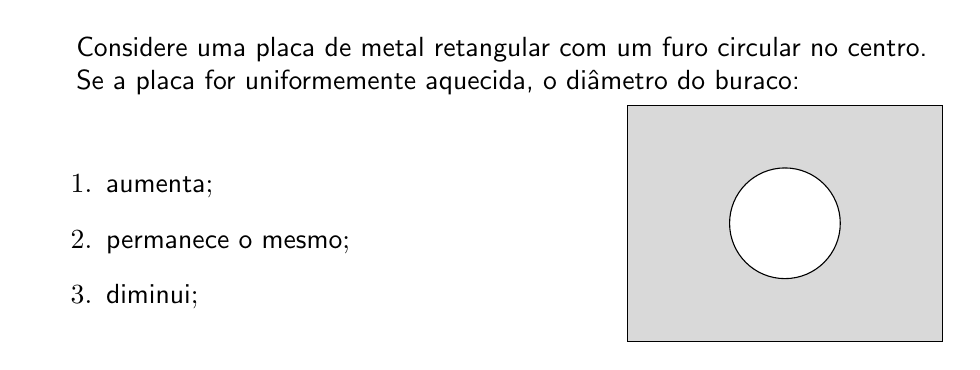
\begin{tikzpicture}[scale=1]
    \label{fig:desenv_ct}
    \node[,text width=11cm] at (0,4) {\textsf{Considere uma placa de metal retangular com um furo circular no centro. Se a
    placa for uniformemente aquecida, o diâmetro do buraco:}};
    \node[,text width=5cm] at (-3.5,2) {
      \begin{enumerate}
        \item \textsf{aumenta};
        \item \textsf{permanece o mesmo};
        \item \textsf{diminui};
      \end{enumerate}
    };
    \draw[fill=gray!30, shift={(1.5cm,.5cm)}](0,0) rectangle (4,3);
    \draw[fill=white, shift={(1.5cm,.5cm)}](2,1.5) circle(20pt);
  \end{tikzpicture}
  \fonte{Adaptado de \cite{Watkins2013}}
\end{figure}

Uma das etapas do IpC na sala de aula é o processo de votação, em que os estudantes
respondem a questões conceituais. Tal processo é associado ao uso de \textit{clickers},
que são pequenos dispositivos trasmissores como na \autoref{fig:desenv_clickers}.

\begin{figure}
  \begin{centering}
    \caption{\label{fig:desenv_clickers}Exemplo de \textit{clickers}}
    \subfloat[\textit{i>clicker 2}]{\includegraphics[scale=0.25]{imagens/desenv_iclicker}}
    \hspace{.5cm}
    \subfloat[\textit{ResponseCard RF LCD}]{\includegraphics[scale=.4517]{imagens/desenv_turning_clicker}}
    \par
  \end{centering}
  \fonte{(a) \href{http://www1.iclicker.com}{iclicker.com} (b) \href{http://www.turningtechnologies.com}{turningtechnologies.com}}
\end{figure}

No entanto, a implementação do IpC não ocorre apenas na sala de aula. Espera-se
que os alunos façam leituras e atividades antes da aula. Também espera-se do
professor guiar os estudantes nessa etapa, seja indicando ou disponibilizando o
material adequado. O tempo em sala de aula que seria utilizado para apenas transferir
informações para os estudante é utilizado principalmente para discussões, interação
entre os estudantes, tempo para assimilação e para pensar  \cite{Mazur2009, Crouch2001}.

\begin{figure}[htbp]
  \centering
  \caption{Diagrama do processo de implementação do método IpC}
  \includegraphics[clip, trim=0cm 18cm 3cm .4cm,scale=0.75]{imagens/peer_instruction}
  \label{fig:desen_fluxograma_ipc}
  \fonte{\cite{X} (Adaptado)}
\end{figure}


\section{Sistemas de Resposta}
\label{section:sistemas_de_resposta}

Com efeito, a tecnologia apresenta-se como meio, como instrumento para colaborar no desenvolvimento do processo de aprendizagem. A tecnologia reveste-se de um valor relativo e dependente desse processo. Ela tem sua importância apenas como um instrumento significativo para favorecer a aprendizagem de alguém. Não é a tecnologia que vai resolver ou solucionar o problema educacional do Brasil. Poderá colaborar, no entanto, se for usada adequadamente, para o desenvolvimento educacional de nossos estudantes.
